From observations of models stability towards different image brightness which are present in the datasets a new hypothesis was drawn. Introducing corruptions that we test on into the training should improve the predictions on corrupted data. Unfortunately it is not possible to use real lab corruptions here as the data was provided only for testing on these difficult cases and was not stained. Without staining one cannot give a quiantitative measure of the quality of the predictions. However, artificial corruptions can be applied here easily. Random changes in contrast, brightness and defocus blur os severity levels $-4$ and $4$ were added to training augmentations. After the improved model was trained the predictions on the corrupted dataset became much better indeed (see Figure \ref{fig:augments-help}).

\begin{figure}[htb]
	\begin{center}
		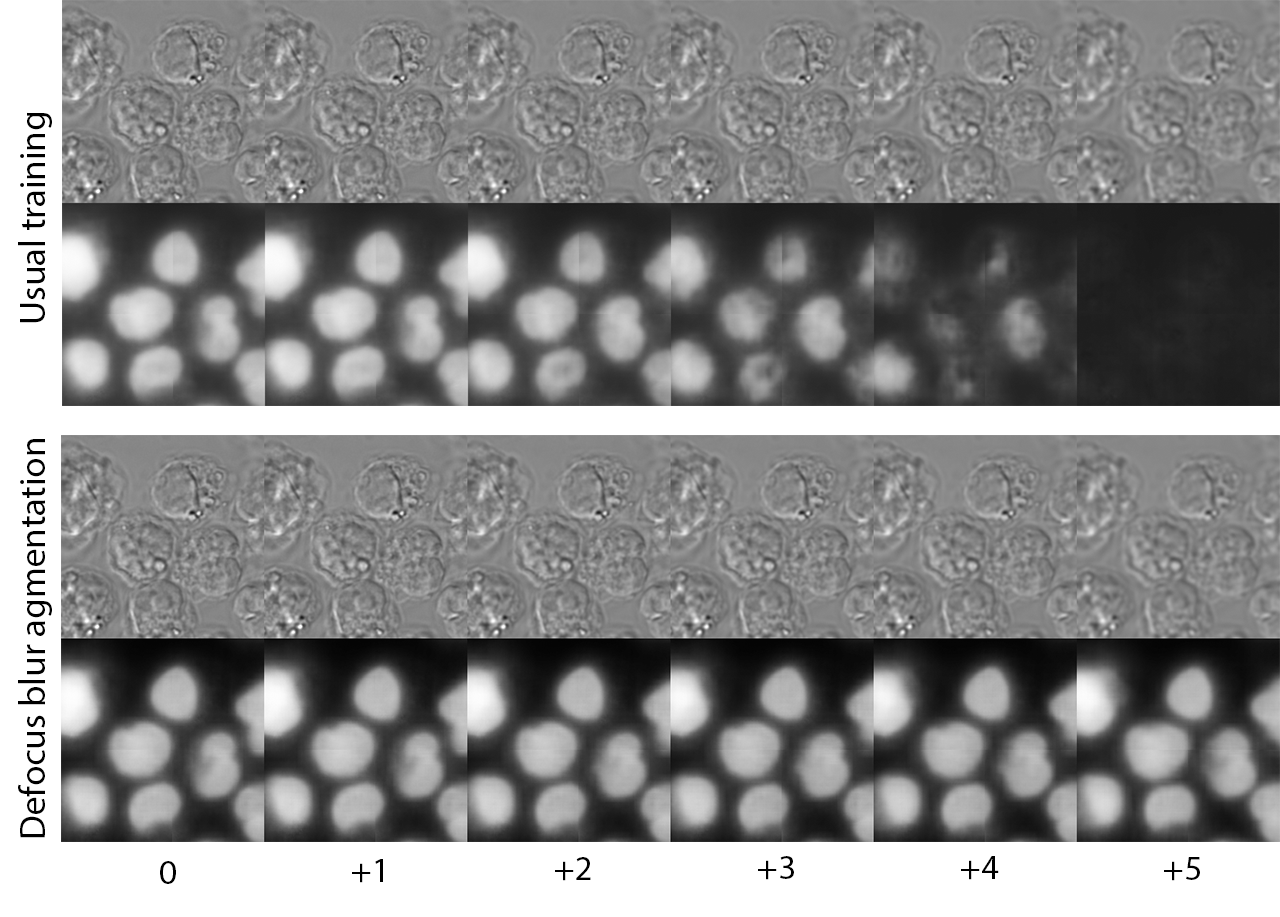
\includegraphics[width=0.8\linewidth]{bilder/stability/augments-help.png}
		\caption{Using corruptions as augmentations improve predictions}\label{fig:augments-help}
	\end{center}
\end{figure}

Additionally, since these corruptions are artifical and the ground truth data from staining is present, the difference in downstream metrics for models with and without augmentations has been measured (see Table TODO). Calculation of downstream metrics remained the same, the only change happened in the input data (artifical corruptions were applied).

TO BE ADDED.

\subsubsection{Influence of corruptions on metrics for downstream tasks}
To be added
Calculate how metrics worsen when the evaluation stays the same, but the input is corrupted.
